\chapter{Discussion}
\label{Discussion}
The following chapter intends to discuss the results of the user study in correlation with comparing the results of the workshop and the card sort. Through this discussion it will be reflected upon how the findings leads to an understanding of the users' mental model.

\section{Comparing the results}
\label{ComparingResults}
As described in \autoref{ChapterWorkshop} is the scope of this user study to explore the users mental model of the TonePrint sharing platform. Which is an important aspect of designing the information architecture. In this pursue, two methods is used separately in order to explore how users group the concepts and functionalities of the platform and how they work together in order use the platform. In a perfect world could the results from this study indicate which content and concepts that should be present in different sites, in order to accommodate the users journey to complete a task. However isn't the world always perfect and the results might be to divers in order to be able to decide on a finished IA yet.

\subsection*{Comparing card sort and individual results}
\label{ComparingIndividualAndCard}
When looking at \autoref{UseOfCardSortData}, \autoref{IndividualTaskReflection} and \autoref{GroupTaskResults} is it very clear that the level of success for the two methods are very different. The results of the card sort is heavily affected by the small sample size and as such lack of qualitative data, whereas the workshop provided a fair amount of data both from the individual tasks which to some extend was comparable, and the discussion when agreeing on a model. The purpose of the individual task was for the subjects to find a TonePrint created by a fictional user. When comparing this task with the results of the card sort the starting point would be to look at the groups focusing on "Finding TonePrints" and the cards representing the concepts and components, that the subjects used in the workshop. As presented in \autoref{IndividualTaskReflection} and the individual models from \autoref{fig:ICMM1} to \autoref{fig:ICMM5}, the first step is to either use a search function or the filtering in the library, in order to locate the corona toneprints created by \textit{User 1}. When looking at cards representing this, such as \textit{TonePrint library}, \textit{Searching system} and \textit{'Effect type' filter}, they are typically located in the search related groups. For the aspect of filtering and searching for another user, \textit{User library} and \textit{'User' filter} are the most prominent cards, but only the filter is seen as a searching tool. Both of these are however grouped as a 'user feed' or 'User Profile', which are concepts that in some way also appear in the workshop results. No cards are directly comparable with the act of finding other users' TonePrints through their profile as some of the subjects proposed in the workshop, but groups labeled 'Profile', 'User setting', and 'User feed' were present. This supports the idea of including a profile site for the users at least to some extend in the TonePrint community. After locating the target TonePrint, highlighting it as a favourite is often the next step followed by downloading and beaming it. While the \textit{TonePrint download system} and \textit{Beaming} cards are sorted together, being identified as TonePrint software tools, the 'favourite part' is more difficult to compare, because no card or group is directly referring to the concept. The cards most related to this is \textit{"Other users also liked this" recommendations}, \textit{'Rating' filter}, \textit{'Popularity' filter} and \textit{User rating system}. The first three of these are always grouped together (When excluding subject 6) however, there is little consistency in the groups they are placed in, the latter card's grouping have nothing in common with the others. A comparison between the two methods for the part of favouring or rating a TonePrint is to far-fetched.

\subsection*{Comparing card sort and group results}
\label{ComparingGroupAndCard}
In the group task, the intention was to have the subjects find a common consensus for how to share a TonePrint, including which concepts and functionalities this should include. As presented in \autoref{GroupTaskResults}, this resulted in a description of a system with somewhat well-defined features. When looking at these results, it's important to remember that they were instructed to include name, description, and tags for categorising the the TonePrint that they had just created. During the discussion of the concept of tags and descriptions, it evident that their arguments are seemingly similar. In the card sort, this is also the case for the \textit{TonePrint category}, \textit{Tags describing a TonePrint} and \textit{TonePrint description} cards which are grouped together every time. These groups either focusses on searching or TonePrints in general. \textit{'Effect type' filter} and \textit{'Genre' filter} are cards that also are grouped with searching, which is quite similar to what is proposed by the group, when discussion what the tags should be based on.  As for the sharing aspect, the group discuss two general concepts, public and private. For the card sort, the cards \textit{Private forum} and \textit{Public forum} are the most similar. These are almost paired by each subject and are grouped in 'Community' groups. This does not indicate that these cards might be related to the concept of sharing one's TonePrint. 
\newpage

\subsection*{General comparison and reflection}
\label{CompareGeneral}
Despite the comparisons above, it is still important to keep in mind that this data stems from a small number of people. This isn't as much a problem for the workshop, given the type of data. It is more a problem for the card sort data. However, some tendencies are spotted, where groups from the card sort, either by label or cards, often are paired together, drawing similarities to concepts or ideas generated in the workshop. This indicates that there might be some common consensus to how the concepts work for e.g filtering or tags and that there is some general idea of a profile being a part of the community. This is however just tendencies spotted in a small set of data hinting at some similarities without statistical evidence. The idea behind conducting the two studies simultaneously was to gather a large amount of data from the card sort, providing a clear indication of conceptual groups, which then would be compared to the conceptualised mental models from the workshop. It's always easy to be skeptical in retrospect when a study doesn't goes as planned. The card sort could have been conducted in-person instead, which would have made it possible to gather more qualitative data, but at the same time, it wouldn't be able to reach users across the globe. A reason for conducting the card sort remote was also that it could "handle itself", allowing time to be allocated to the workshop and other aspects of the project.\\

\noindent
When reflecting on the workshop there's also some perspective worth taking to consideration. The results derived from the individual tasks are based on five users' ability to conceptualise and verbalise how they wants to solve a task, using an imaginary system. The number of participants of course limits how much that might be derived from the workshop alone, however it is still possible to find tendencies with only few subject, when using qualitative methods. When subjects conceptualise their mental models for a task, the findings are also limited to the extent of that task. An example from this study is that there seems to be a general idea of the concept of profiles. Because the task denotes that the subjects should locate a TonePrint, the only information derived for the profile is that it contains the TonePrints created by that user. This doesn't mean that the users lack a mental model regarding what the profile concept also might include, it just indicates that the their mental model of the profile concept tells them that it can be used to access that user's TonePrints. Instead of using the task focused approach, the subjects could just have been told to \textit{Name the concepts you think should be a part of the TonePrint sharing platform, and describe these concepts}. By doing that, the task limitations are avoided, however, this could result in the subjects providing superficial descriptions because they lack a context to base it on. In order to reach the entire extend of the platform more studies should be conducted and even then would it be far-fetched to state that the entire mental model has been explored. \\

\noindent
Compared with the individual tasks, the group task provides a more thorough description of the concepts used to complete the task, because the subjects are describing and discussing their understanding of the concept in order to reach a common consensus in the group. It could be argued that both tasks of the workshop should be conducted as group tasks in order to get a more thorough description of the concepts for the first task. However, it is also possible that the group task went well, because the subjects already have framed their mindset towards creating concepts and verbalised them through the presentation, which means that each subject in the group task already was in a state of mind that may have affected the group discussion. If another workshop was to be conducted it should be considered to switch the task around, making the upload task individual and having it as the first and the task of finding a TonePrint last, as a group task.\\

\section{The mental model (for now)}
\label{MentalModelForNow}
The results derived from \autoref{CardSortAnalysis} and \autoref{WorkshopResults} have been compared and reflected upon in \autoref{ComparingResults}, and now it's time to use that information. As described in \autoref{ChapterWorkshop} the aim of the user study is to explore the users' mental model of the TonePrint community.\\ 
Through this study, it's found that the TonePrint community should include a searching functionality which enables the user to find TonePrints by searching or filtering in a list by \textit{Effect type}, \textit{name}, \textit{user name}, \textit{parameters} of the TonePrint described as tags, and which ever \textit{tag} assigned to a TonePrint. There should be user profiles which are accessible though the search functionality. The profile should include the TonePrints that the respective users have defined as public and maybe some personal remarks and descriptions. The TonePrints should include \textit{descriptions}, highlights the user's intentions with the TonePrint and maybe describe the settings of it. The TonePrint should also include tags that describes the parameters and effect type of the TonePrint, where some of them suggested to the user based on the TonePrint parameters and description by the system, and some is created entirely by the user. It should be possible to download the TonePrint to one's own unit and add it to a favourite list. The TonePrints is either \textit{private} and can't be accessed by others, it can be \textit{unlisted} which only is accessible for specific other users granted access, or it can be \textit{public} for everyone to access. A conceptualised model of the TonePrint, based on the description above is presented on \autoref{fig:ConcludingModel}.

This mental model does not depict the entire community with all its concepts and content, so to accommodate this, new studies should be conducted focusing on both specific concepts e.g how tags should be based on the parameters and how they are understood by the users, or specific groupings of content e.g what content should be on the same page and how should i be structured hierarchically. Based on the findings of this study, a new card sort could be conducted with cards representing examples of content that belongs to the concepts displayed on \autoref{fig:ConcludingModel}. This could be a closed card sort using the concepts as predefined groups. The results would then show to what extend, the concepts are understandable. Another approach could be to create a Low-fidelity prototype based on this model, which then could be used to have the users conducting simple tasks, exploring how the model derived from this study is interpreted by other users. Both approaches help exploring the understanding of the model in order to elaborate on it and create a design accommodating the mental model. 
%
\begin{figure}[H]
	\centering
	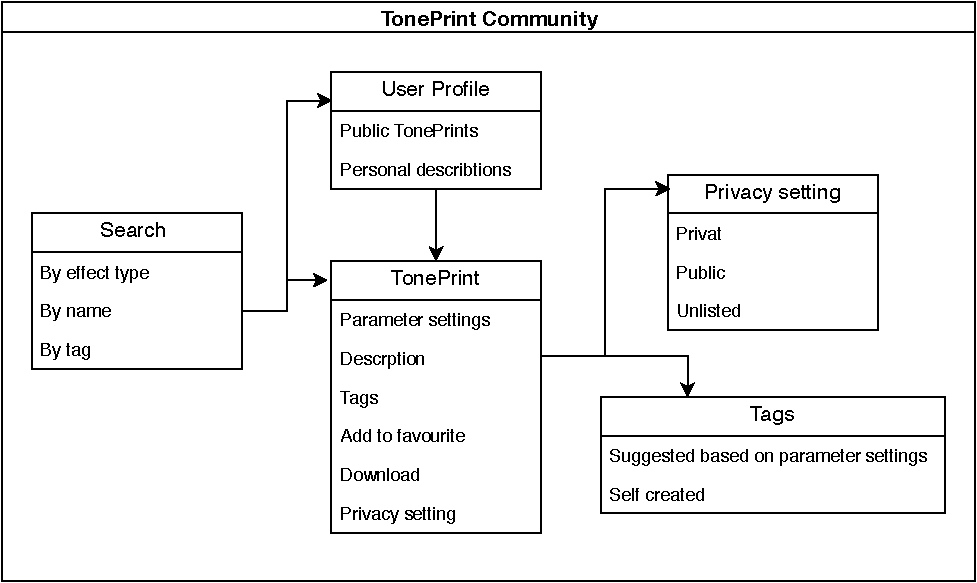
\includegraphics[width=0.7\textwidth]{ConcludingModel.pdf}
	\caption{The conceptualized Mental Model}
	\label{fig:ConcludingModel}
\end{figure}
%
